
\documentclass[12pt]{article}
\usepackage[english]{babel}
\usepackage{float}
\usepackage[margin=1in]{geometry}
\usepackage{graphicx}
%\usepackage[toc,page]{appendix}
\graphicspath{ {./img/} }
\newcommand{\rpm}{\raisebox{.2ex}{$\scriptstyle\pm$}} 
\usepackage{listings}
\usepackage{xcolor}
\usepackage{indentfirst}
\usepackage[final]{pdfpages}


\begin{document}

\title{Joe Phaneuf \\ Computer Vision 16-720 Spring 2018 \\ Feb. 03, 2018 }
\date{}
\author{}
%\maketitle



\section{Theory Questions}

\subsection{Q2.1  }
Mapping a point in image space $(x,y)$ to Hough space, $x$ and $y$ become constants.  
$\rho(\theta) = x cos \theta + y sin \theta$  
Being a linear combination of same-period sinusoids, $\rho(\theta)$ is guaranteed to be a sinusoid.  

\subsection{Q2.2  }
Hough space can be parameterized in slope-intercept form.  
Doing so creates two major problems:  

\subsubsection{The slope and intercept parameters are unbounded, making implementation impractical}

\subsubsection{Vertical lines (infinite slope) cannot be represented  }

When parameterizing in normal form, the magnitude and angle are bounded (magnitude bound is a function of image size).

$\rho = x cos \theta + y sin \theta$  
$y sin \theta = \rho - x cos \theta$  
$y = - \frac{1}{tan \theta} x + \frac{\rho}{sin \theta}$  
$m =- \frac{1}{tan \theta}$ , $c = \frac{\rho}{sin \theta}$  

\subsection{Q2.3  }
The range of $\theta$ is independent on image size: $- \frac{\pi}{2} \leq \theta \leq \frac{\pi}{2}$  
The largest $\rho$ will be a diagonal across the image space: $0 \leq abs(\rho) \leq \sqrt{W^{2} + H^{2}}$

\subsection{Q2.4  }
\subsubsection{ Matlab script for plot generation in matlab/q2.4.m}
Image space points (10, 10), (15, 15) and (30, 30) were represented in Hough space, resulting in sinusoids as discussed above. The sinusoids in Hough space intersect at one point. That point describes a line in image space that passes through the points (10, 10), (15, 15) and (30, 30). The sinusoids intersect at $\theta = - \frac{pi}{4}$ , $\rho = 0$, which describes a 45 degree line passing through origin in image space, i.e. $m=1$, $c=0$.



\begin{figure}[H]
\centering
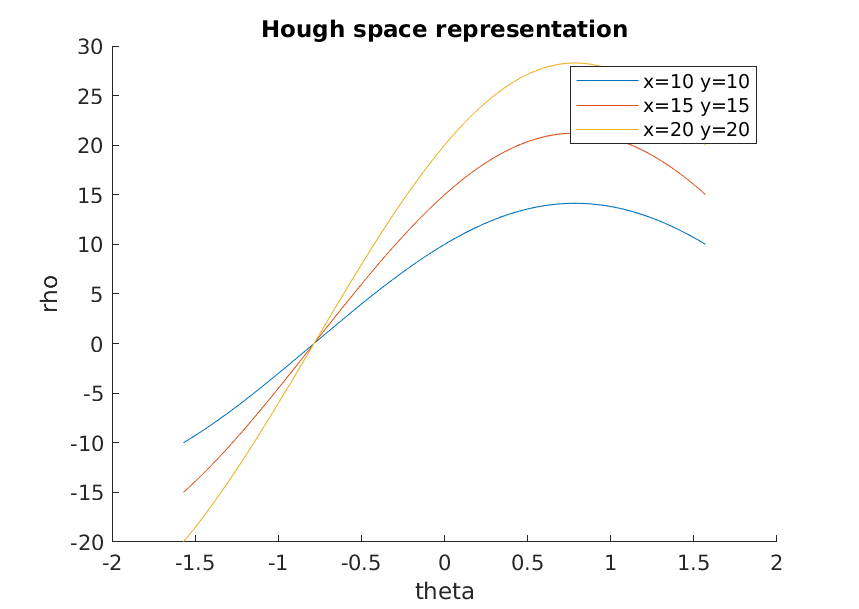
\includegraphics[page=1,width=0.75\textwidth]{q2_4}
\caption{Intersecting lines in Hough space}    
\label{fig:bblr}
\end{figure}   


\subsection{Q2.5  }
Extra Credit

\section{Implementation}

\subsection{3.1}
\subsection{3.2}
\subsection{3.3}
\subsection{3.4}
\subsection{3.5}
\subsection{3.6}

\section{Experiments}
\subsubsection{Did your code work well on all the image with a single set of parameters? }

I was unable to find a single set of parameters that performered equally well across all images. In particular
Best image 1:
sigma: 1.000000
threshold: 0.250000
rhoRes: 1.000000
thetaRes: 1.000000
nLines: 50.000000

Best/cleanest on images 6 and 9
sigma: 3.000000
threshold: 0.100000
rhoRes: 1.000000
thetaRes: 0.500000
nLines: 50.000000

\subsection{4.1 How did the optimal set of parameters vary with images? }
After experimenting on 10 parameter sets, the gaussian filter standard deviation parameter appears to have the most impact on image to image variation. Experiments with lower standard deviation showed better results for images with clearly defined lines and little noise (such as image 1), however noisier images (such as image 6 and image 9) had noisy responses.
Increasing the standard deviation of the gaussian filter results in cleaner lines on noisy images, but resulted in fewer detected lines on less noisy images.

\subsection{4.2 Which step of the algorithm causes the most problems? }
From these results I would argue the the edge filter is the most problematic piece of this process, as a fixed blur causes inconsistent results across images with wildly different frequency content.

\subsection{4.3 Did you find any changes you could make to your code or algorithm that improved performance?}
I found maintaining single for loops / vectorization to provide faster performance when batch processing images.

\subsection{4.4 Tabulate the different experiments that you have performed with their results in your write-up.}

\subsection{4.5 Also de-scribe how well your code worked on different images, what effect the parameters had on any improvements that you made to your code to make it work better. }
Images with non-linear elements (such as image 2 with the vase and image 6 with the text on boxes) consistently resulted in inaccurate lines. Increasing the edge threshold resulted in fewer but more accurate lines on these images.

\subsection{4.6 If you made changes to your code that required changes to the results generation script, include your updated version in your submission.  }
It's not required to run, but I modified the script to save results to a new timestamped directory with the parameters written to a text file. This made it easier to keep track of all experiments, would be a nice-to-add feature for future homeworks like this for non-Matlabians.

\newpage


\section{Team Goals}

\end{document}
